\documentclass[10pt]{article}
\usepackage[margin=0.85in]{geometry}
\usepackage{amsmath,amssymb,amsthm}
\usepackage{graphicx}
\usepackage{caption}
\captionsetup{font=small}

\newtheorem{proposition}{Proposition}

\newcommand{\supIPM}{\mathrm{supIPM}}
\newcommand{\EIPM}{\mathrm{EIPM}}
\newcommand{\hsupIPM}{\widehat{\supIPM}}
\newcommand{\Wone}{W_1}

\pagestyle{empty}
\begin{document}

\begin{center}\vspace{-0.5em}
{\large\bfseries Experiment}
\vspace{-0.5em}\end{center}


\section{Simulation 1}

\paragraph{Purpose.} Two things. \emph{(1)} The motivation for using the supremum. \emph{(2)} Our estimator $\hsupIPM$ recovers the true
$\supIPM$.

\begin{proposition}
For a joint law $P$ of $(S,Z)$ with $S$ absolutely continuous, let
$\Delta_P(s) = \sup_{f \in \mathrm{Lip}_1} \big| \mathbb E_P[f(Z) \mid S{=}s] - \mathbb E_P[f(Z)] \big|$.
For every $\varepsilon, M > 0$ there is such a $P$, with $S \sim N(0,1)$ and
$\operatorname{Var}_P(Z) = 1$, satisfying
\[
\mathbb E_P\big[\Delta_P(S)\big] \;\le\; \varepsilon
\qquad\text{and}\qquad
\operatorname*{sup}_{s} \Delta_P(s) \;\ge\; M .
\]
\end{proposition}

\noindent The converse inequality is trivial, so $\supIPM$ is a strictly stronger guarantee.


\paragraph{Data.}
\[
S \sim N(0,1), \qquad Z \mid S{=}s \sim N\!\big(\mu(s),\,\sigma_c^2\big),
\qquad \mu(s) = \kappa\exp\!\Big(\!-\tfrac{(s-s_0)^2}{2\tau^2}\Big),
\qquad \kappa = 1.2,\ \ s_0 = 0.7,\ \ \tau = 0.2,
\]
with $\sigma_c^2 = 1 - \operatorname{Var}(\mu(S))$ so that $\operatorname{Var}(Z) = 1$. 

\paragraph{Estimator.} For a fixed $s$, weight each observation by how close $s_i$ is to $s$, and
compare the resulting conditional distribution to the pooled one:
\[
\widehat F_s(u) = \sum_i w_i(s)\,\mathbf 1(z_i \le u), \qquad
w_i(s) = \frac{K_h(s-s_i)}{\sum_j K_h(s-s_j)}, \qquad
\widehat \Wone(s) = \int \big|\widehat F_s(u) - \widehat F(u)\big|\,du ,
\]
with $K_h$ a Gaussian kernel of bandwidth $h$ and $\widehat F$ the pooled empirical CDF. 
We use $h = 0.25\,n^{-1/5}$, grid spacing $h/2$, and $n = 500,\dots,2{\times}10^4$ with $100$
replications each.

\paragraph{Why this design.} With a $\mathrm{Lip}_1$ discriminator $\mathrm{IPM} = \Wone$, and for
one-dimensional $Z$ the truth is available in closed form, so the estimator can be checked against
it. This setting makes $\supIPM$ large while $\EIPM$ stays small.



% \paragraph{What we measure.} The estimated curve $\widehat \Wone(\cdot)$ against the truth, and the
% error of $\hsupIPM$ against the rate $n^{-2/5}$. The curve matters because
% $|\max_s \widehat \Wone - \max_s \Wone| \le \|\widehat \Wone - \Wone\|_\infty$ --- a supremum is
% reliable only if the estimate is close everywhere.

\paragraph{Result.} 
The followings are result.
\begin{figure}[!h]\vspace{-0.5em}
\centering
    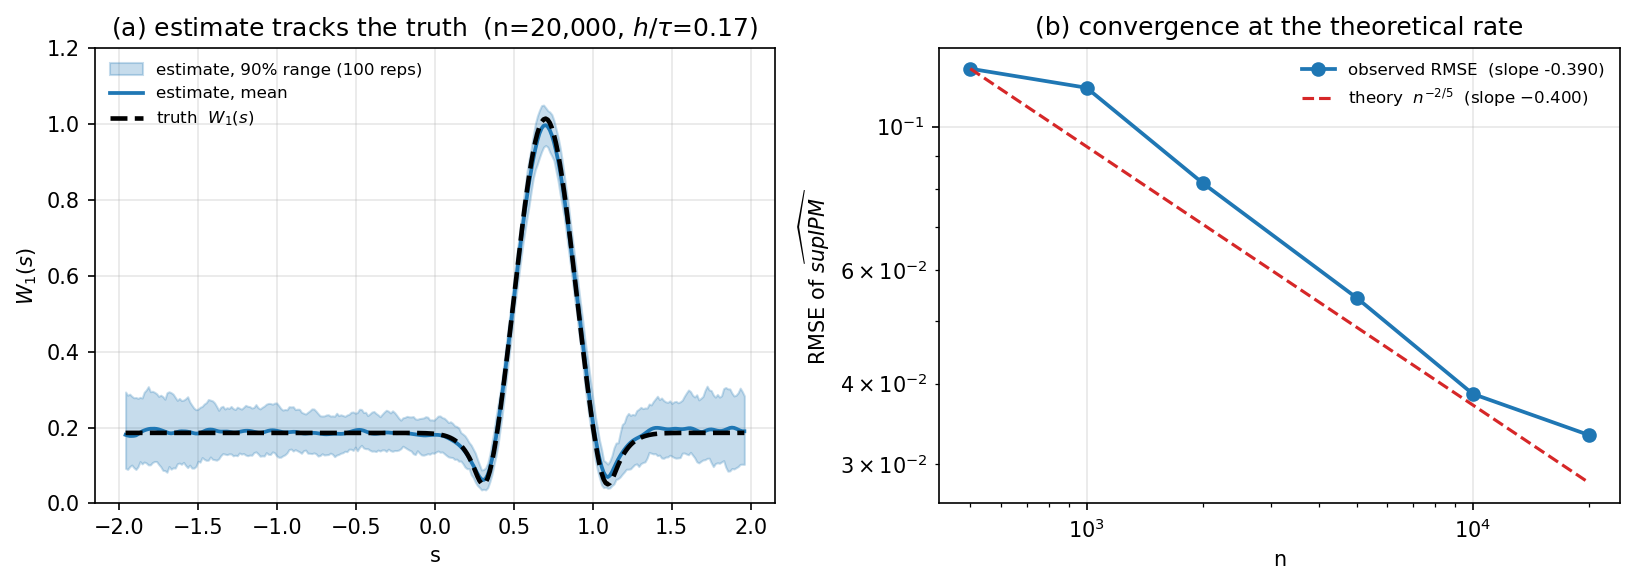
\includegraphics[width=1\linewidth]{figures//Simulation/S1_main.png}
\caption{(a) $\widehat{W_1}(s)$ against the truth
($n = 2{\times}10^4$). (b) RMSE of $\hsupIPM$ vs.\ $n$, with the theoretical
$n^{-2/5}$ line.}
\end{figure}
\vspace{-0.5em}


% \paragraph{Result.} The estimate tracks the truth uniformly in $s$, recovers both the peak and its
% location, and converges at the theoretical rate. The bandwidth must stay below the bump width $\tau$
% for this to hold: a wider kernel averages over a window larger than the bump, flattening the peak, and
% the rate is not attained --- as expected, since the expansion $\mathrm{bias} = O(h^2)$ presumes
% $h < \tau$. The resulting bias is always negative, so an oversized bandwidth reports the
% representation as \emph{fairer} than it is. Since $\tau$ is unknown in real data, how to choose $h$
% remains open.

\end{document}